\documentclass{beamer}
%\usepackage[latin1]{inputenc}
%\usepackage{lmodern}
\usepackage{times}
\usepackage[T1]{fontenc}
\usepackage{graphicx}
\usepackage{bm}
\usepackage{tikz}
\usepackage{verbatim}
\usepackage{amsmath}
\usepackage[small,labelformat=empty]{caption}
\usepackage{url}
\usetikzlibrary{automata,positioning}

\usetheme{Frankfurt}
%\usetheme{Warsaw}
\title[Title of presentation]{Uhrenbaustein\\
{\small Time&Date and Countdown}
}
\author[author name]
{Tobias F{\"u}lle}
\institute[Fnord GmbH]{Lehrstuhl f{\"u}r integrierte Systeme}
\date{Tue - 06/11/12}

\begin{document}

%{
%\usebackgroundtemplate{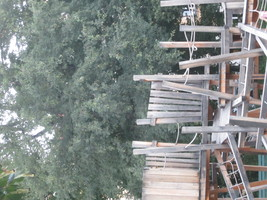
\includegraphics[width=\paperwidth]{pictures/sample.jpg}}
%\begin{frame}
%\thispagestyle{empty}
%\titlepage
%\end{frame}
%%}
%%
%\begin{frame}
%\frametitle{Overview}
%\tableofcontents
%\end{frame}
%
%\setlength\fboxsep{5pt}
%\setlength\fboxrule{0pt}

\section{Time and Date}



  \begin{frame}{Circuit diagram}  
  	\begin{figure}
  		\centering
  		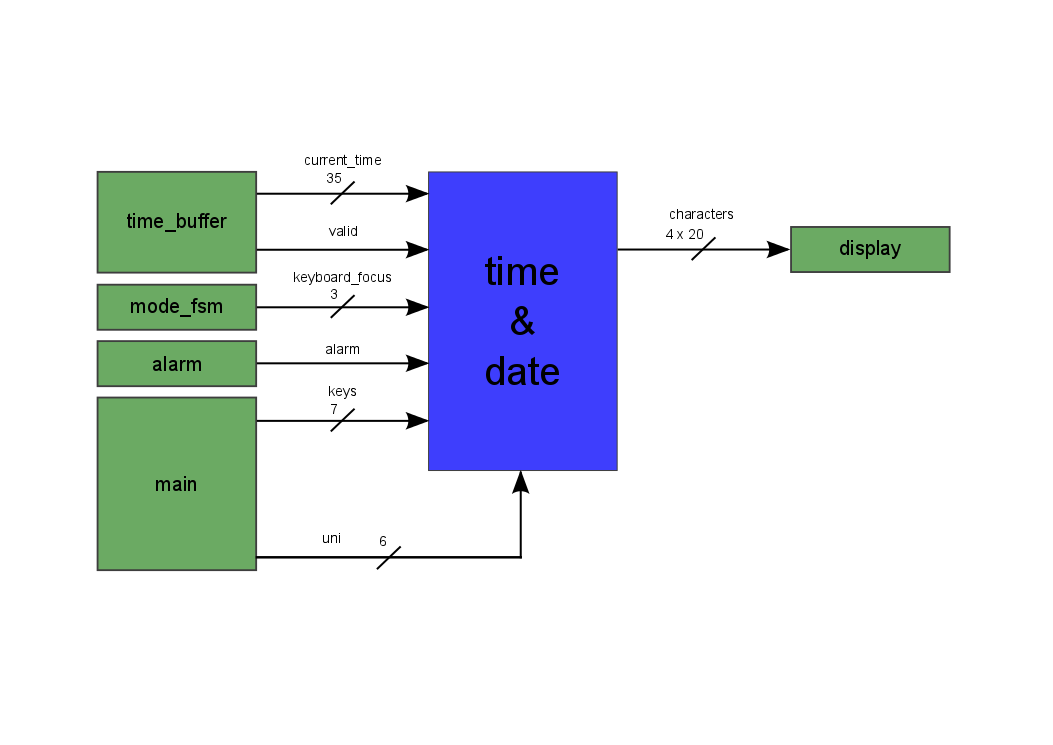
\includegraphics[scale=0.35]{Zeichnung.png}
  	\end{figure}
  \end{frame}

  \begin{frame}{FSM  state diagram}
  	\begin{figure}
    	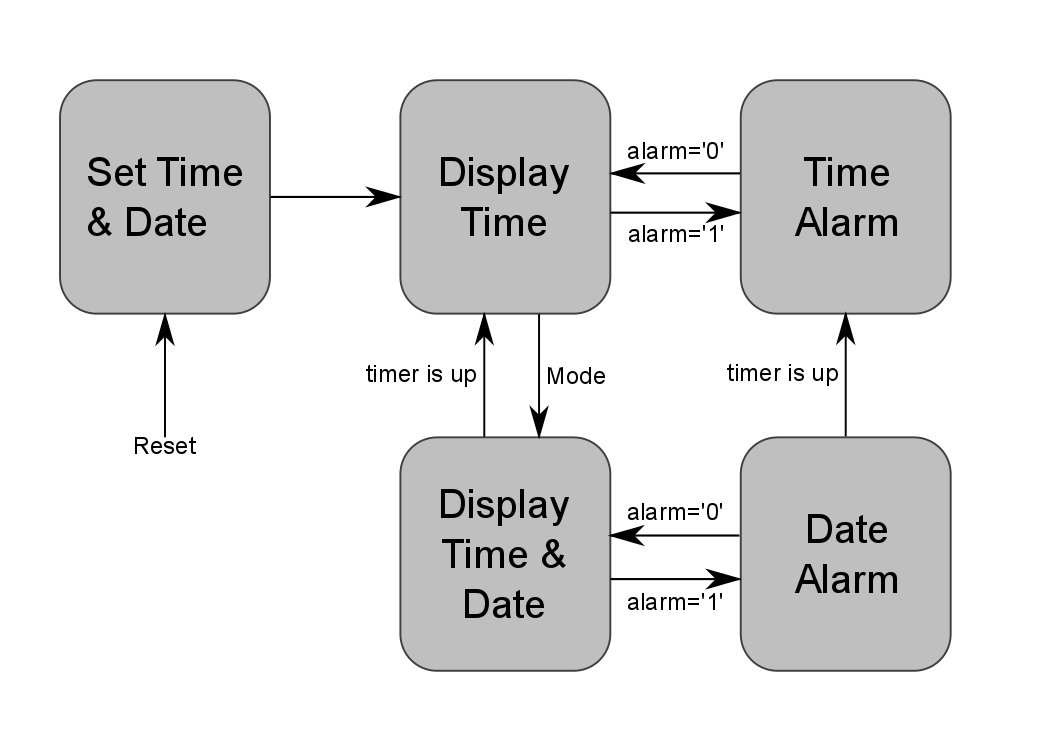
\includegraphics[scale=0.35]{Tdsd.png}
    \end{figure}
  \end{frame}

\section{Countdown}

  \begin{frame}{Circuit diagram}
  	\begin{figure}
  		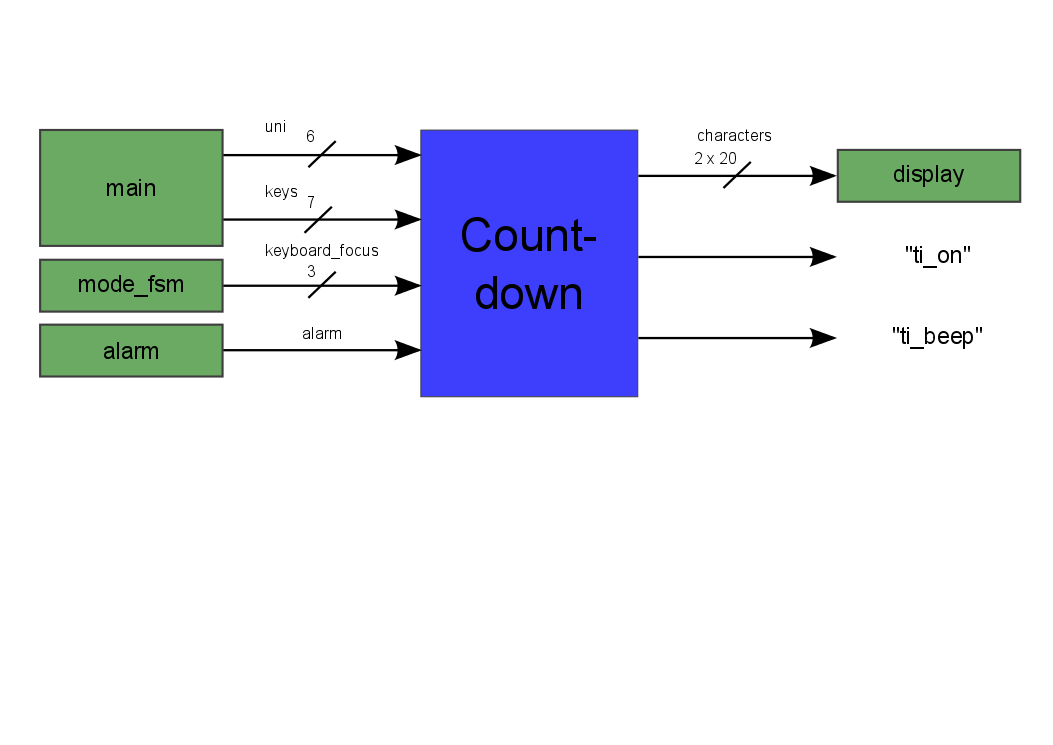
\includegraphics[scale=0.35]{Countdown.png}
  	\end{figure}
  \end{frame}

  \begin{frame}{FSM  state diagram}
  	\begin{figure}
   		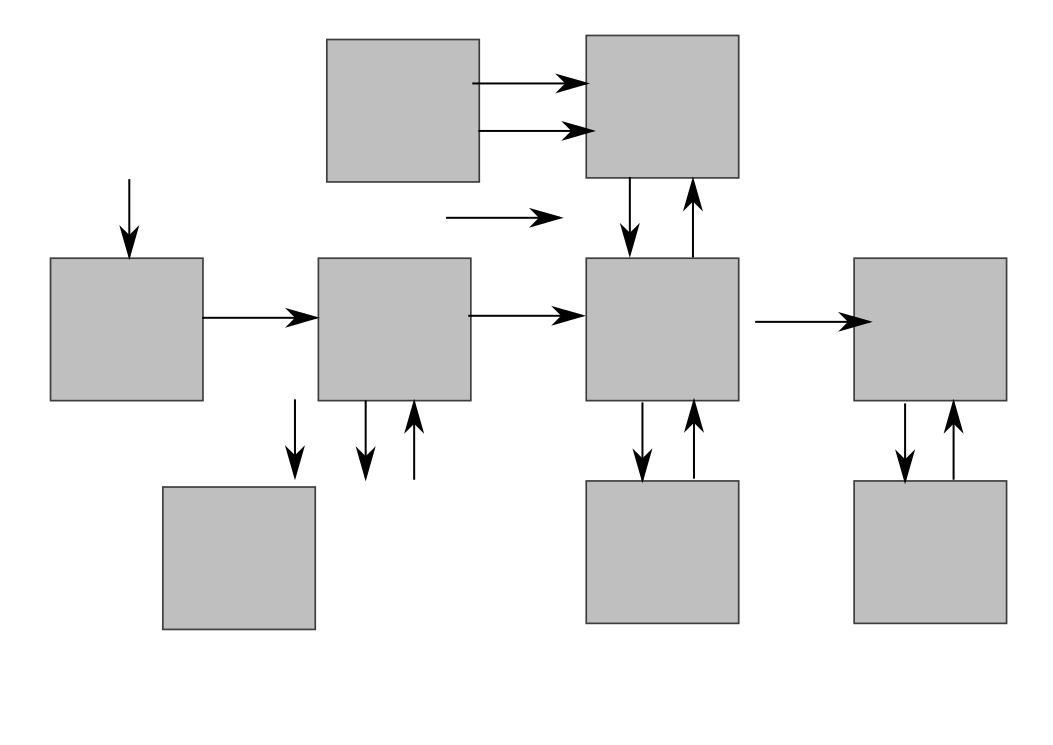
\includegraphics[scale=0.35]{Cdsd.png}
    \end{figure}
  \end{frame}
%  
\end{document}

